
%% bare_conf.tex
%% V1.3
%% 2007/01/11
%% by Michael Shell
%% See:
%% http://www.michaelshell.org/
%% for current contact information.
%%
%% This is a skeleton file demonstrating the use of IEEEtran.cls
%% (requires IEEEtran.cls version 1.7 or later) with an IEEE conference paper.
%%
%% Support sites:
%% http://www.michaelshell.org/tex/ieeetran/
%% http://www.ctan.org/tex-archive/macros/latex/contrib/IEEEtran/
%% and
%% http://www.ieee.org/

%%*************************************************************************
%% Legal Notice:
%% This code is offered as-is without any warranty either expressed or
%% implied; without even the implied warranty of MERCHANTABILITY or
%% FITNESS FOR A PARTICULAR PURPOSE! 
%% User assumes all risk.
%% In no event shall IEEE or any contributor to this code be liable for
%% any damages or losses, including, but not limited to, incidental,
%% consequential, or any other damages, resulting from the use or misuse
%% of any information contained here.
%%
%% All comments are the opinions of their respective authors and are not
%% necessarily endorsed by the IEEE.
%%
%% This work is distributed under the LaTeX Project Public License (LPPL)
%% ( http://www.latex-project.org/ ) version 1.3, and may be freely used,
%% distributed and modified. A copy of the LPPL, version 1.3, is included
%% in the base LaTeX documentation of all distributions of LaTeX released
%% 2003/12/01 or later.
%% Retain all contribution notices and credits.
%% ** Modified files should be clearly indicated as such, including  **
%% ** renaming them and changing author support contact information. **
%%
%% File list of work: IEEEtran.cls, IEEEtran_HOWTO.pdf, bare_adv.tex,
%%                    bare_conf.tex, bare_jrnl.tex, bare_jrnl_compsoc.tex
%%*************************************************************************

% *** Authors should verify (and, if needed, correct) their LaTeX system  ***
% *** with the testflow diagnostic prior to trusting their LaTeX platform ***
% *** with production work. IEEE's font choices can trigger bugs that do  ***
% *** not appear when using other class files.                            ***
% The testflow support page is at:
% http://www.michaelshell.org/tex/testflow/



% Note that the a4paper option is mainly intended so that authors in
% countries using A4 can easily print to A4 and see how their papers will
% look in print - the typesetting of the document will not typically be
% affected with changes in paper size (but the bottom and side margins will).
% Use the testflow package mentioned above to verify correct handling of
% both paper sizes by the user's LaTeX system.
%
% Also note that the "draftcls" or "draftclsnofoot", not "draft", option
% should be used if it is desired that the figures are to be displayed in
% draft mode.
%
\documentclass[conference]{IEEEtran}
% Add the compsoc option for Computer Society conferences.
%
% If IEEEtran.cls has not been installed into the LaTeX system files,
% manually specify the path to it like:
% \documentclass[conference]{../sty/IEEEtran}





% Some very useful LaTeX packages include:
% (uncomment the ones you want to load)


% *** MISC UTILITY PACKAGES ***
%
%\usepackage{ifpdf}
% Heiko Oberdiek's ifpdf.sty is very useful if you need conditional
% compilation based on whether the output is pdf or dvi.
% usage:
% \ifpdf
%   % pdf code
% \else
%   % dvi code
% \fi
% The latest version of ifpdf.sty can be obtained from:
% http://www.ctan.org/tex-archive/macros/latex/contrib/oberdiek/
% Also, note that IEEEtran.cls V1.7 and later provides a builtin
% \ifCLASSINFOpdf conditional that works the same way.
% When switching from latex to pdflatex and vice-versa, the compiler may
% have to be run twice to clear warning/error messages.






% *** CITATION PACKAGES ***
%
%\usepackage{cite}
% cite.sty was written by Donald Arseneau
% V1.6 and later of IEEEtran pre-defines the format of the cite.sty package
% \cite{} output to follow that of IEEE. Loading the cite package will
% result in citation numbers being automatically sorted and properly
% "compressed/ranged". e.g., [1], [9], [2], [7], [5], [6] without using
% cite.sty will become [1], [2], [5]--[7], [9] using cite.sty. cite.sty's
% \cite will automatically add leading space, if needed. Use cite.sty's
% noadjust option (cite.sty V3.8 and later) if you want to turn this off.
% cite.sty is already installed on most LaTeX systems. Be sure and use
% version 4.0 (2003-05-27) and later if using hyperref.sty. cite.sty does
% not currently provide for hyperlinked citations.
% The latest version can be obtained at:
% http://www.ctan.org/tex-archive/macros/latex/contrib/cite/
% The documentation is contained in the cite.sty file itself.






% *** GRAPHICS RELATED PACKAGES ***
%
\ifCLASSINFOpdf
  \usepackage[pdftex]{graphicx}
  \usepackage{subfigure}
  % declare the path(s) where your graphic files are
  \graphicspath{{./fig/}{../jpeg/}}
  % and their extensions so you won't have to specify these with
  % every instance of \includegraphics
  % \DeclareGraphicsExtensions{.pdf,.jpeg,.png}
\else
  % or other class option (dvipsone, dvipdf, if not using dvips). graphicx
  % will default to the driver specified in the system graphics.cfg if no
  % driver is specified.
  % \usepackage[dvips]{graphicx}
  % declare the path(s) where your graphic files are
  %\graphicspath{{./fig/}}
  % and their extensions so you won't have to specify these with
  % every instance of \includegraphics
  % \DeclareGraphicsExtensions{.eps}
\fi
% graphicx was written by David Carlisle and Sebastian Rahtz. It is
% required if you want graphics, photos, etc. graphicx.sty is already
% installed on most LaTeX systems. The latest version and documentation can
% be obtained at: 
% http://www.ctan.org/tex-archive/macros/latex/required/graphics/
% Another good source of documentation is "Using Imported Graphics in
% LaTeX2e" by Keith Reckdahl which can be found as epslatex.ps or
% epslatex.pdf at: http://www.ctan.org/tex-archive/info/
%
% latex, and pdflatex in dvi mode, support graphics in encapsulated
% postscript (.eps) format. pdflatex in pdf mode supports graphics
% in .pdf, .jpeg, .png and .mps (metapost) formats. Users should ensure
% that all non-photo figures use a vector format (.eps, .pdf, .mps) and
% not a bitmapped formats (.jpeg, .png). IEEE frowns on bitmapped formats
% which can result in "jaggedy"/blurry rendering of lines and letters as
% well as large increases in file sizes.
%
% You can find documentation about the pdfTeX application at:
% http://www.tug.org/applications/pdftex





% *** MATH PACKAGES ***
%
\usepackage[cmex10]{amsmath}
\usepackage{amssymb}
\usepackage{amsmath}
\usepackage{amsfonts}
% A popular package from the American Mathematical Society that provides
% many useful and powerful commands for dealing with mathematics. If using
% it, be sure to load this package with the cmex10 option to ensure that
% only type 1 fonts will utilized at all point sizes. Without this option,
% it is possible that some math symbols, particularly those within
% footnotes, will be rendered in bitmap form which will result in a
% document that can not be IEEE Xplore compliant!
%
% Also, note that the amsmath package sets \interdisplaylinepenalty to 10000
% thus preventing page breaks from occurring within multiline equations. Use:
%\interdisplaylinepenalty=2500
% after loading amsmath to restore such page breaks as IEEEtran.cls normally
% does. amsmath.sty is already installed on most LaTeX systems. The latest
% version and documentation can be obtained at:
% http://www.ctan.org/tex-archive/macros/latex/required/amslatex/math/

\newtheorem{definition}{Definition}
\newtheorem{theorem}{Theorem}
%\newtheorem{proof}{Proof}
\newtheorem{lemma}{Lemma}
\newtheorem{assumption}{Assumption}
\newtheorem{proposition}{Proposition}
\newtheorem{example}{Example}





% *** SPECIALIZED LIST PACKAGES ***
%
\usepackage{algorithmic}
\usepackage{algorithm}
% algorithmic.sty was written by Peter Williams and Rogerio Brito.
% This package provides an algorithmic environment fo describing algorithms.
% You can use the algorithmic environment in-text or within a figure
% environment to provide for a floating algorithm. Do NOT use the algorithm
% floating environment provided by algorithm.sty (by the same authors) or
% algorithm2e.sty (by Christophe Fiorio) as IEEE does not use dedicated
% algorithm float types and packages that provide these will not provide
% correct IEEE style captions. The latest version and documentation of
% algorithmic.sty can be obtained at:
% http://www.ctan.org/tex-archive/macros/latex/contrib/algorithms/
% There is also a support site at:
% http://algorithms.berlios.de/index.html
% Also of interest may be the (relatively newer and more customizable)
% algorithmicx.sty package by Szasz Janos:
% http://www.ctan.org/tex-archive/macros/latex/contrib/algorithmicx/




% *** ALIGNMENT PACKAGES ***
%
%\usepackage{array}
% Frank Mittelbach's and David Carlisle's array.sty patches and improves
% the standard LaTeX2e array and tabular environments to provide better
% appearance and additional user controls. As the default LaTeX2e table
% generation code is lacking to the point of almost being broken with
% respect to the quality of the end results, all users are strongly
% advised to use an enhanced (at the very least that provided by array.sty)
% set of table tools. array.sty is already installed on most systems. The
% latest version and documentation can be obtained at:
% http://www.ctan.org/tex-archive/macros/latex/required/tools/


%\usepackage{mdwmath}
%\usepackage{mdwtab}
% Also highly recommended is Mark Wooding's extremely powerful MDW tools,
% especially mdwmath.sty and mdwtab.sty which are used to format equations
% and tables, respectively. The MDWtools set is already installed on most
% LaTeX systems. The lastest version and documentation is available at:
% http://www.ctan.org/tex-archive/macros/latex/contrib/mdwtools/


% IEEEtran contains the IEEEeqnarray family of commands that can be used to
% generate multiline equations as well as matrices, tables, etc., of high
% quality.


%\usepackage{eqparbox}
% Also of notable interest is Scott Pakin's eqparbox package for creating
% (automatically sized) equal width boxes - aka "natural width parboxes".
% Available at:
% http://www.ctan.org/tex-archive/macros/latex/contrib/eqparbox/





% *** SUBFIGURE PACKAGES ***
%\usepackage[tight,footnotesize]{subfigure}
% subfigure.sty was written by Steven Douglas Cochran. This package makes it
% easy to put subfigures in your figures. e.g., "Figure 1a and 1b". For IEEE
% work, it is a good idea to load it with the tight package option to reduce
% the amount of white space around the subfigures. subfigure.sty is already
% installed on most LaTeX systems. The latest version and documentation can
% be obtained at:
% http://www.ctan.org/tex-archive/obsolete/macros/latex/contrib/subfigure/
% subfigure.sty has been superceeded by subfig.sty.



%\usepackage[caption=false]{caption}
%\usepackage[font=footnotesize]{subfig}
% subfig.sty, also written by Steven Douglas Cochran, is the modern
% replacement for subfigure.sty. However, subfig.sty requires and
% automatically loads Axel Sommerfeldt's caption.sty which will override
% IEEEtran.cls handling of captions and this will result in nonIEEE style
% figure/table captions. To prevent this problem, be sure and preload
% caption.sty with its "caption=false" package option. This is will preserve
% IEEEtran.cls handing of captions. Version 1.3 (2005/06/28) and later 
% (recommended due to many improvements over 1.2) of subfig.sty supports
% the caption=false option directly:
%\usepackage[caption=false,font=footnotesize]{subfig}
%
% The latest version and documentation can be obtained at:
% http://www.ctan.org/tex-archive/macros/latex/contrib/subfig/
% The latest version and documentation of caption.sty can be obtained at:
% http://www.ctan.org/tex-archive/macros/latex/contrib/caption/




% *** FLOAT PACKAGES ***
%
%\usepackage{fixltx2e}
% fixltx2e, the successor to the earlier fix2col.sty, was written by
% Frank Mittelbach and David Carlisle. This package corrects a few problems
% in the LaTeX2e kernel, the most notable of which is that in current
% LaTeX2e releases, the ordering of single and double column floats is not
% guaranteed to be preserved. Thus, an unpatched LaTeX2e can allow a
% single column figure to be placed prior to an earlier double column
% figure. The latest version and documentation can be found at:
% http://www.ctan.org/tex-archive/macros/latex/base/



%\usepackage{stfloats}
% stfloats.sty was written by Sigitas Tolusis. This package gives LaTeX2e
% the ability to do double column floats at the bottom of the page as well
% as the top. (e.g., "\begin{figure*}[!b]" is not normally possible in
% LaTeX2e). It also provides a command:
%\fnbelowfloat
% to enable the placement of footnotes below bottom floats (the standard
% LaTeX2e kernel puts them above bottom floats). This is an invasive package
% which rewrites many portions of the LaTeX2e float routines. It may not work
% with other packages that modify the LaTeX2e float routines. The latest
% version and documentation can be obtained at:
% http://www.ctan.org/tex-archive/macros/latex/contrib/sttools/
% Documentation is contained in the stfloats.sty comments as well as in the
% presfull.pdf file. Do not use the stfloats baselinefloat ability as IEEE
% does not allow \baselineskip to stretch. Authors submitting work to the
% IEEE should note that IEEE rarely uses double column equations and
% that authors should try to avoid such use. Do not be tempted to use the
% cuted.sty or midfloat.sty packages (also by Sigitas Tolusis) as IEEE does
% not format its papers in such ways.
\DeclareMathOperator*{\argmax}{arg\,max}




% *** PDF, URL AND HYPERLINK PACKAGES ***
%
%\usepackage{url}
% url.sty was written by Donald Arseneau. It provides better support for
% handling and breaking URLs. url.sty is already installed on most LaTeX
% systems. The latest version can be obtained at:
% http://www.ctan.org/tex-archive/macros/latex/contrib/misc/
% Read the url.sty source comments for usage information. Basically,
% \url{my_url_here}.





% *** Do not adjust lengths that control margins, column widths, etc. ***
% *** Do not use packages that alter fonts (such as pslatex).         ***
% There should be no need to do such things with IEEEtran.cls V1.6 and later.
% (Unless specifically asked to do so by the journal or conference you plan
% to submit to, of course. )


% correct bad hyphenation here
\hyphenation{op-tical net-works semi-conduc-tor}


\begin{document}
%
% paper title
% can use linebreaks \\ within to get better formatting as desired
%\title{Locate multiple ultrasound emitters on unique frequency simultaneously}
\title{On locating multiple ultrasound emitter in chorus}

% author names and affiliations
% use a multiple column layout for up to three different
% affiliations
%\author{Lei Song, IIIS}
\author{\IEEEauthorblockN{Lei Song}
\IEEEauthorblockA{NEC Labs China\\
Beijing, China \\
Email:Song\_lei@nec.cn}
\and
\IEEEauthorblockN{Yongcai Wang}
\IEEEauthorblockA{IIIS, Tsinghua University\\
   Beijing, China \\
Email: wangyc@tsinghua.edu.cn}
}

% conference papers do not typically use \thanks and this command
% is locked out in conference mode. If really needed, such as for
% the acknowledgment of grants, issue a \IEEEoverridecommandlockouts
% after \documentclass

% for over three affiliations, or if they all won't fit within the width
% of the page, use this alternative format:
% 
%\author{\IEEEauthorblockN{Michael Shell\IEEEauthorrefmark{1},
%Homer Simpson\IEEEauthorrefmark{2},
%James Kirk\IEEEauthorrefmark{3}, 
%Montgomery Scott\IEEEauthorrefmark{3} and
%Eldon Tyrell\IEEEauthorrefmark{4}}
%\IEEEauthorblockA{\IEEEauthorrefmark{1}School of Electrical and Computer Engineering\\
%Georgia Institute of Technology,
%Atlanta, Georgia 30332--0250\\ Email: see http://www.michaelshell.org/contact.html}
%\IEEEauthorblockA{\IEEEauthorrefmark{2}Twentieth Century Fox, Springfield, USA\\
%Email: homer@thesimpsons.com}
%\IEEEauthorblockA{\IEEEauthorrefmark{3}Starfleet Academy, San Francisco, California 96678-2391\\
%Telephone: (800) 555--1212, Fax: (888) 555--1212}
%\IEEEauthorblockA{\IEEEauthorrefmark{4}Tyrell Inc., 123 Replicant Street, Los Angeles, California 90210--4321}}




% use for special paper notices
%\IEEEspecialpapernotice{(Invited Paper)}




% make the title area

\maketitle

\begin{abstract}
%\boldmath
Although TOA based positioning by narrow-band ultrasound is not fairly new as research
problem, there are still some open questions. In this paper, an interesting issue, that
how to locate multiple ultrasound transmitters simultaneously, is addressed.  This
problem is difficult because of two reasons. Firstly, Two segments of ultrasound wave on
same frequency, if overlapped in time-domain at receiver end, can not be separated
efficiently.  Secondly, the emitter of narrow-band ultrasound signal can not be
identified on the receiver end.  To avoid collision and anonymity, emitters are arranged
to non-overlapped timeslot in traditional TOA based positioning system. The disadvantage
of timeslot based mechanism is obvious, that the refreshing rate drops when number of
timeslot increase.  In this paper, we reduce the number of timeslots by allowing
multiple emitters to send ultrasound signal simultaneously. Although the collision and
anonymity of ultrasound signal are still inevitable at receiver end, the position of
each emitter can be estimated by assigning the incomplete TOA measurement to several
groups and adjust the assignment according to make distance measurements in each group
are consistent with each other. As the feasible assignment is exponential to number of emitter,
which are intractable to go through, importance sampling and particle filter is used to
reduce the number of feasible assignment by taking historical position of each emitter
into account. This method is named \emph{UltraChorus} because emitter can ``sing''
concurrently. The performance of UltraChorus is evaluated by multi-agent simulation.
\end{abstract}
% IEEEtran.cls defaults to using nonbold math in the Abstract.
% This preserves the distinction between vectors and scalars. However,
% if the conference you are submitting to favors bold math in the abstract,
% then you can use LaTeX's standard command \boldmath at the very start
% of the abstract to achieve this. Many IEEE journals/conferences frown on
% math in the abstract anyway.

% no keywords

% For peer review papers, you can put extra information on the cover
% page as needed:
% \ifCLASSOPTIONpeerreview
% \begin{center} \bfseries EDICS Category: 3-BBND \end{center}
% \fi
%
% For peerreview papers, this IEEEtran command inserts a page break and
% creates the second title. It will be ignored for other modes.
\IEEEpeerreviewmaketitle

\section{Introduction}
Using narrow-band ultrasound pulse (NUP) as ranging media for TOA positioning is
popular in wireless sensor network, because only basic I/O ability on
transmitter/receiver is required to get TOA measurement of high precision. In
corresponding system, an ultrasound pulse is generated by transmitter and caught by
receiver. By measuring the propagation time of the wave-front, the distance between
transmitter and receiver can be obtained in centimeter level\cite{Priyantha:2000hx}.
With measured distances the position of emitter can be located if the location of
receivers are known.  In last decade, there are a lot of research focusing on this
topic. In other word, so far, there are quite few thing we can do to improve the
performance of narrow-band ultrasound in positioning system except some open issues.
Among these issues, the contradict between number of supported emitters and positioning
refreshing rate is a interesting one.  

In narrow-band ultrasound signal based positioning system, two or more ultrasound
transmitters are not allowed to emit signal at the same time. There are two reasons why
this constrains exits. First reason is referred as \emph{anonymity} of ultrasound
signal. Because there are no room to encode information into a narrow-band ultrasound
pulse, receiver can not identify the source of a segment of ultrasound wave. The second
reason is referred as \emph{collision} of ultrasound signal. When two or more segments
of ultrasound wave from different transmitter overlaps in time domain on the receiver.
Only the wave-front of the first one can be identified, while the wave-front of the
other are lost. In this case, the number of TOA measurement is less than the number of
transmitters.  

Because of this two reasons, in previous NUP based positioning systems, such as bat and
cricket,   transmitters are designed to work in TDMA protocol. In this case, in time
slot occupied by $i$th transmitter, all the receivers only caught one pulse from $i$th
transmitter, therefore the drawback of anonymity and collision is eliminated. But in
the other hand, the refresh-rate of location  drops linearly to the number of emitter
supported in this system. A trade-off between system capacity and positioning delay has
to be made.

Facing this issue, some research use encoded braodband ultrasound to replace NUP. Both
\emph{anonymity} and {collision} are resolved by employing CDMA technology into both
transmitter and receiver\cite{Hazas:2006tv}. To achieve encoding and decoding, high
performance MCU or DSP is required, which increase the cost and reduce the batter-life.
Some research try to use the AOA( angle of arrival) as compensate to increase the
spatial resolution of receiver to tackle the simultaneously arrived
pulse\cite{Yu:2009ix}. Both of these method required extra sensor of computing unit. 

In this paper a new method to process simultaneously arrived ultrasound pulse is
presented.  The basic idea is that we doesn't increase the sensing ability of existing
system such as cricket and bat, although they produce incomplete  measurement when
emitters start to work simultaneously. All we want to do is infer the location of target
by post-processing on incomplete measurement.  More specially, we infers feasible
location of each target and find the set of location with maximum likelihood as
estimation result. In this process, we reduce the complexity of finding feasible
location by involving estimated location of emitters in previous instant as
prior-knowledge. 

The rest part of this paper is organized as follows, in section 2 the formal statement
of problem addressed in this paper is presented. In section 3, the method named
\emph{UltraChorus} is proposed as solution to NUP based multi-emitter locating problem. 
In section 4, the method is evaluated by simulation.
% that's all folks
\section{Problem modeling}
The system component of TOA based positioning system working in timeslot is illustrated in
figure \ref{fig:1ToN}. $m$ receivers are deployed in fixed spot, whose position is denoted
by $X(R_i),i\in[1,m]$. $n$ mobile emitter can move freely, whose position is denoted
by $X_t(T_i),i\in[1,n]$ at instant $t$. In timeslot occupied by $i$th emitter, emitter
$i$ transmit the NUP and a radio signal at exactly the same time. Each receiver can catch
the NUP and radio signal. By measuring the arrival time difference between NUP and radio signal.
The distance between $T_i$ and $R_j,j\in[1,m]$, which is denoted by
$D_t(T_i,R_j),j\in[1,m]$, can be obtained in one time slot. Briefly, in time slot mode,
$m$ distance can be obtained in one time slot. The origin of all distance is $T_i$.
Based on $D_t(T_i,R_j),j\in[1,m]$ and $X(R_j),j\in[1,m]$, $X(T_i)$ can be calculated. 
As a result, for $m$ emitter, $m$ time slot is required to locate all emitter with
certainty.

\begin{figure}
    \subfigure[Working in timeslot]{
	\label{fig:1ToN} %% label for first subfigure
	\begin{minipage}[b]{0.22\textwidth}
	    \centering
	    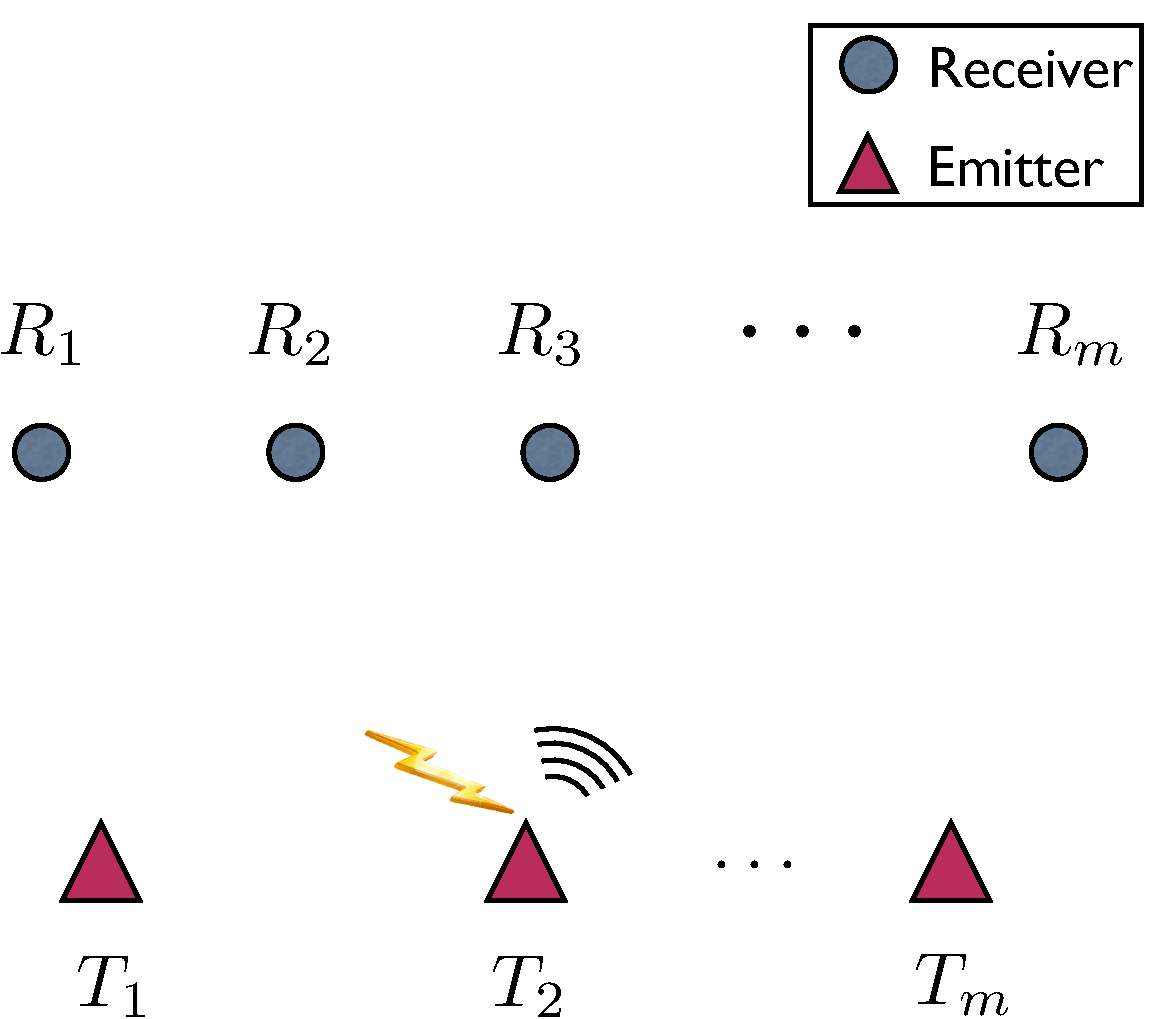
\includegraphics[width=\textwidth]{1ToN}
	\end{minipage}
    }
    \hspace{.02\textwidth}
    \subfigure[Working in chorus]{
	\label{fig:NToN} %% label for second subfigure
	\begin{minipage}[b]{0.22\textwidth}
	    \centering
	    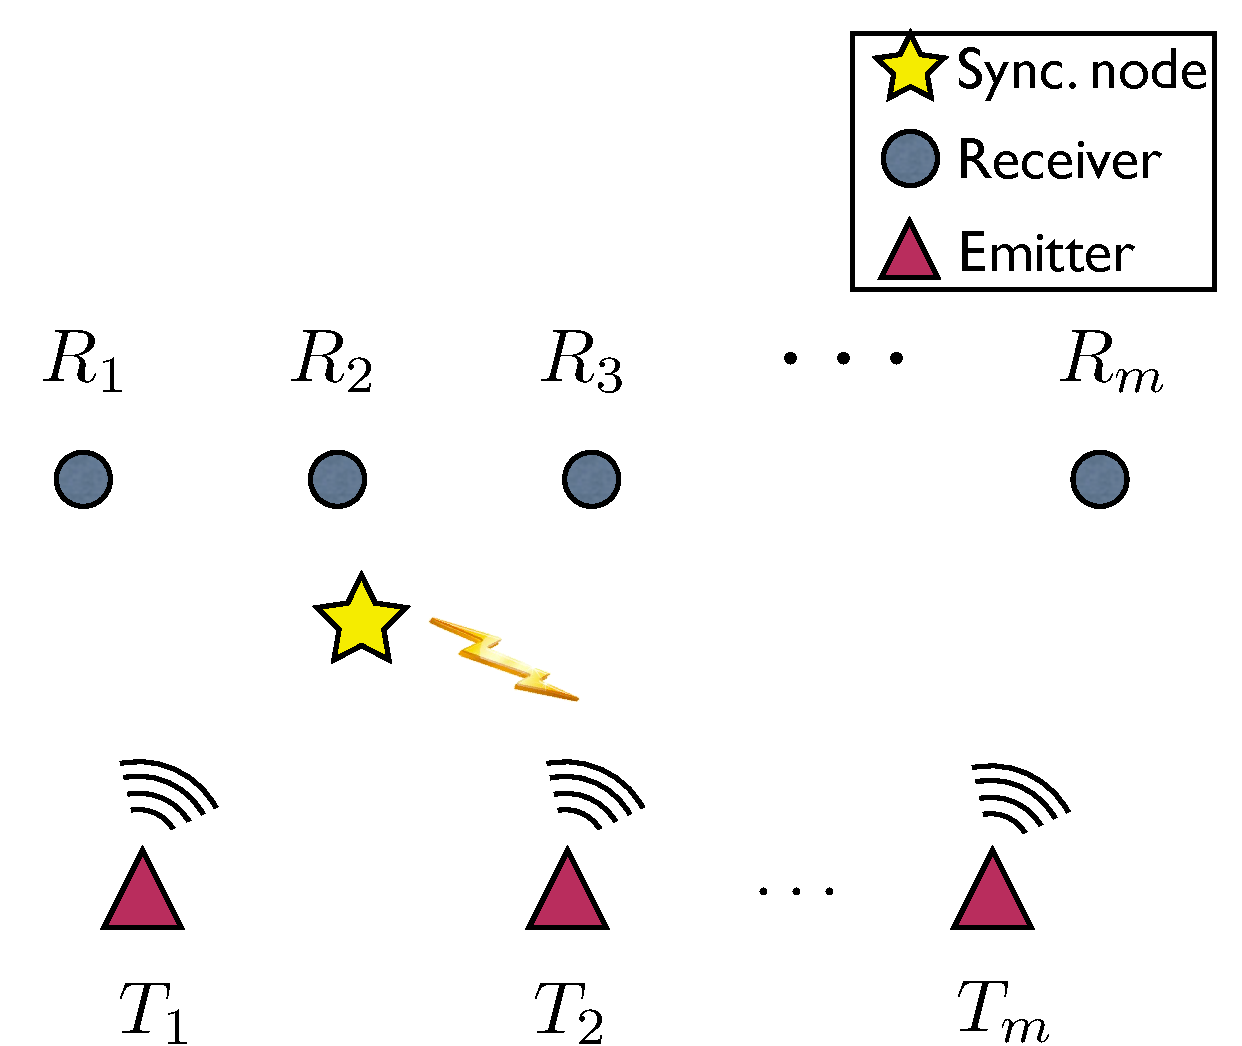
\includegraphics[width=\textwidth]{NtoN}
	\end{minipage}}
    \caption{The system architecture of TOA Based positioning system working on
    different mode}
    \label{fig:systemcomponents} %% label for entire figure
\end{figure}

When system working in chorus mode, the system architecture is shown in figure
\ref{fig:NToN}. A new component, sync node, is added to the system. Once the sync node
broadcast a radio signal at instance $t$, all receivers, $\{T_1,T_2,\dots,T_m\}$, emit
the NUP simultaneously. In ideal case, on any receiver $R_i$, $m$ UDP from
$T_i,i\in[1,m]$ are pairwise isolated in time domain, therefore we can obtain $n$
distance from receiver $R_i$. Because the total number of receivers is $m$, $m\cdot n$
distance, $D(R_i,T_j),i\in[1,m],j\in[1,n]$, can be obtained at instance $t$. 

Although the working in chorus mode can greatly improve the number of distance obtained
in one time slot, the \emph{anonymity} and \emph{collision} is inevitable. Even in the
ideal mode, because the origin of each distance is unknown, we had to assign the $mn$
distance measurement into $m$ subgroup before positioning. We can find all possible
assignment within $n$ round. At round $j$, we choose one out of $m$ distance reported
by each receiver and put them into subgroup $j$. After $n$ round, the $mn$ distance is
separated into $m$ subgroup. We can apply positioning algorithm on each subgroup to get
feasible position for each emitter. The number of different assignment is 
\begin{equation}
    N_a=m!^{n-1}
    \label{equ:assign}
\end{equation}

Because the distance in one subgroup are not always consist with each other and can not
produce valid position estimation. Most of the assignment are not feasible. But is
intractable to go through $N_a$ assignment to find the most feasible one. Briefly, the
\emph{anonymity} can introduce complexity that can not be tolerated.

In unideal state, the UDP on each receiver can not be separated in time domain. Because
only the first wave-front can be detected, some distance measurement are lost. As a
result the distance we can get in one timeslot is less than $mn$ but greater than $m$.
Briefly, the distance set is incomplete due to the \emph{collision} happened in receiver
end.

Taking both \emph{collision} issue and \emph{anonymity} issue into account, the formal
statement of problem addressed in this paper comes as follow. 

\emph{Give:} location of receivers, $X(R_i),i\in[1,n]$, and incomplete distance measurement
$\tilde{D}_t\subset\{D(R_i,T_j),i\in[1,m]\}$ at instant $t$. 

\emph{Ensure:} let $\mathbf{X}_t(T_{1:m})$ denote the location of $m$ emitters
at instant $t$. Then we want to find the maximum likelihood estimation to
$\mathbf{X}_t(T_{1:m})$ condition on $\tilde{D}_t$, 
\begin{equation}
    \hat{\mathbf{X}}_t(T_{1:m})=\argmax_{\mathbf{X}_t(T_{1:m})} p(\mathbf{X}_t(T_{1:m})|\tilde{D}_t)
    \label{equ:ML}
\end{equation}
The brutal force algorithm to solve equation \ref{equ:ML} is to go through $N_a$
possible assignment. With each assignment, we can get a candidate for
$\mathbf{X}_t(T_{1:m})$ 

\section{Analysis and Algorithm}
Determined by the character of NUP, only incomplete and anonymous distance measurement
can be obtained on receiver. In this section the character of distance obtained on
receiver is analyzed. Although information is not sufficient to locate each emitter
directly, we found that solution space of equation \ref{equ:ML} can be reduced greatly and
solution with maximum likelihood can be found with high probability. 

\subsection{limitation of distance measurement}
As discussed in last section, the incomplete is caused by the overlapping of NUP on
receiver end. As shown in figure \ref{fig:overlap}, let $t_w$ denote the width of a NUP
and  $t_\Delta$ denote the arrival time difference of two successive NUP. When
$t_\Delta\le t_w$, they overlap. To reduce the probability of overlap, the width of NUP
should be as small as possible.
\begin{figure}[htpb]
    \begin{center}
	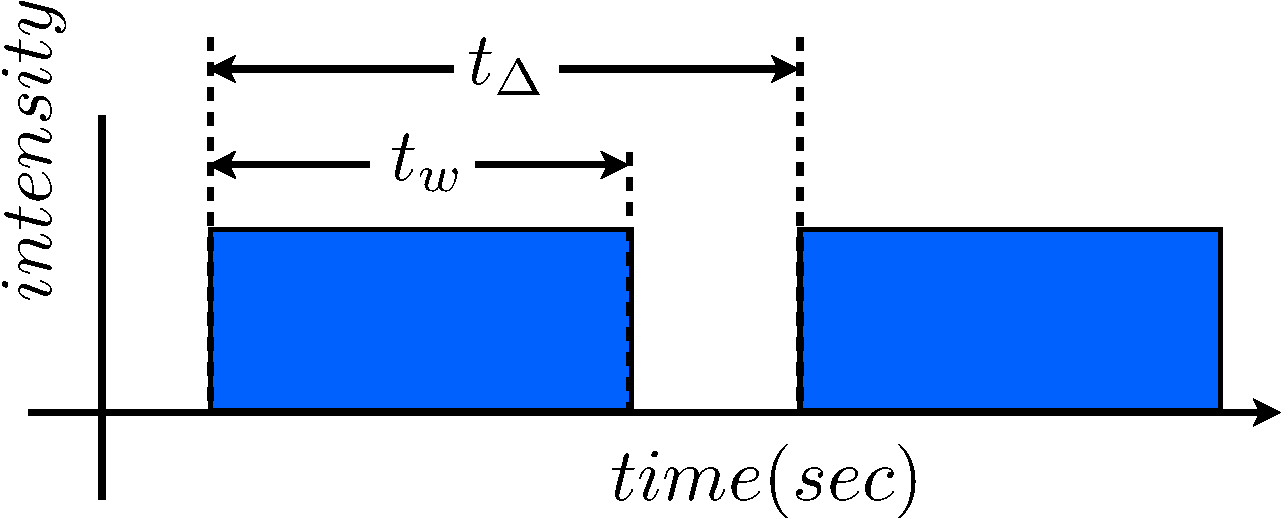
\includegraphics[width=.25\textwidth]{overlap}
    \end{center}
    \caption{Two successive NUP are overlapped if the interval is less than width }
    \label{fig:overlap}
\end{figure}
 
In practice, the $t_w$ is determined by the length of NUP from emitter and the length of
aftershock on receiver end. We measured these two length on  Cricket
node\cite{Priyantha:2000hx} with oscilloscope. The result is shown in figure
\ref{fig:OSC}, in which the upper channel is the wave captured at emitter and the lower
channel is the wave captured at receiver end. At emitter end, the length of NUP is about
$100\mu s$, while in receiver end this length is about $5ms$. This experiment show that
the $t_w$ in Cricket is about $5ms$, any two successive NUP with interval
shorter than $5ms$ overlaps with each other. As the NUP is only $100\mu s$ at emitter
side, the $5ms$ NUP at receiver is mainly aftershock. As the aftershock is decided by
the sensing character of device, $t_w$ can be considered as a constant. 
\begin{figure}[htpb]
    \begin{center}
    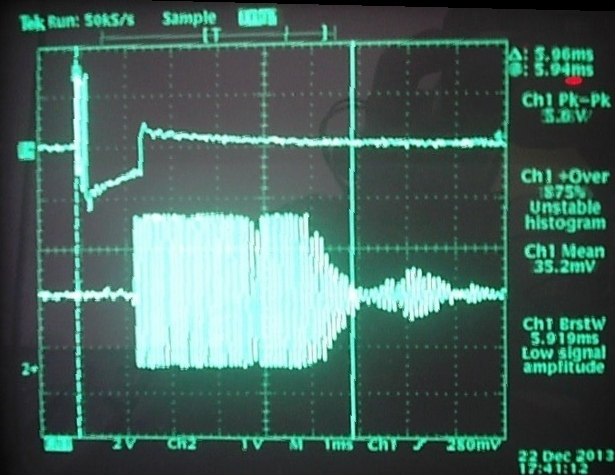
\includegraphics[width=.3\textwidth]{OSC}
    \caption{The NUP on emitter and receiver}
    \label{fig:OSC}
    \end{center}
\end{figure}
Obviously ranging error caused by overlapping is upper bounded by $t_w \times V_u$, if
overlapping of 3 or more NUP never happens. Here $V_u$ is the velocity of ultrasound.
Here we constrains the number of overlapping NUP to guarantee maximum width of
overlapped NUP. How to achieve this ``at most 2'' constrains will be explained later. 
Taking $t_w$ in Cricket node and $V_u$ in normal condition as example, $t_w V_u=1.65m$.

\subsection{Limit of emitters' movement }
Although the motion of emitter is unpredictable, their trajectory still satisfy 
basic criteria, says the trajectory of emitter is continuous in spatial.
Therefore the location of emitter at $t$ is more close to its location at $t-1$ than the
location of other emitter at time $t-1$. I.e., following equation holds,
\begin{equation}
    \begin{split}
	&\forall j\in[1,m],j\ne i\\
	&p(||X_t(T_i)-X_{t-1}(T_i)||<||X_t(T_i)-X_{t-1}(T_j)||)=1-\delta
    \end{split}
    \label{equ:closeto}
\end{equation}
where $\delta$ is a small positive number. With equation \ref{equ:closeto}, we can draw
the conclusion that positions of $T_i$ at $t$ and $t-1$ are close with high probability.
Especially, if a emitter is attached to an object whose maximum velocity known, then
$||X_t(T_i)-X_{t-1}(T_i)||$ is upper bounded by positioning interval times maximum
velocity with high probability. i.e. $X_t(T_i)$ is in a circle with high probability,
whose center is $X_{t-1}(T_i)$ and radius is $r_i$. Here $r_i$ is determined by sampling
interval and velocity of $T_i$. 

\subsection{Location algorithm}
By combining limit of distance measurement and of emitters' movement, we can limit the
feasible arrangement. As shown in figure \ref{fig:LimitToArrange}. The feasible
$X_t(T_i)$ is limited to circle $(X_{t-1}(T_i), \alpha), \alpha=V_e\cdot\Omega$, while
$V_e$ is the upper bounder of emitter's velocity. For each receiver $R_j$,there are must
be a distance $D_t(R_j,T_i)$ from receiver $R_j$ can reach a point in cycle
$(X_t(T_i),\beta),\beta=V_u\cdot T_w$. As a result, following theorem holds.
\begin{theorem}
    For any emitter $T_i$, given $X_t(T_i)$ and $\tilde{D}_t$. There must be a set of distance 
    $\{\tilde{d}_t^j\}\subset \tilde{D}_t,j\in[1,n]$. Such that $\forall
    j\in[1,n]$, $\tilde{d}_t^j$ has one end in $X{R_i}$ and the other ender can
    reach circle $(X_{t-1}(T_i),\alpha+\beta)$ 
    \label{Thm:limit}
\end{theorem}
\begin{proof}
Apply limit of distance measurement and limit of emitters' movement together.
For each receiver, there must exists one distance measurement with one end
fixed on $R_i$ and the other end can reach big circle $(X_{t-1}(T_i),\alpha+\beta)$
\end{proof}

\begin{figure}[htpb]
    \begin{center}
	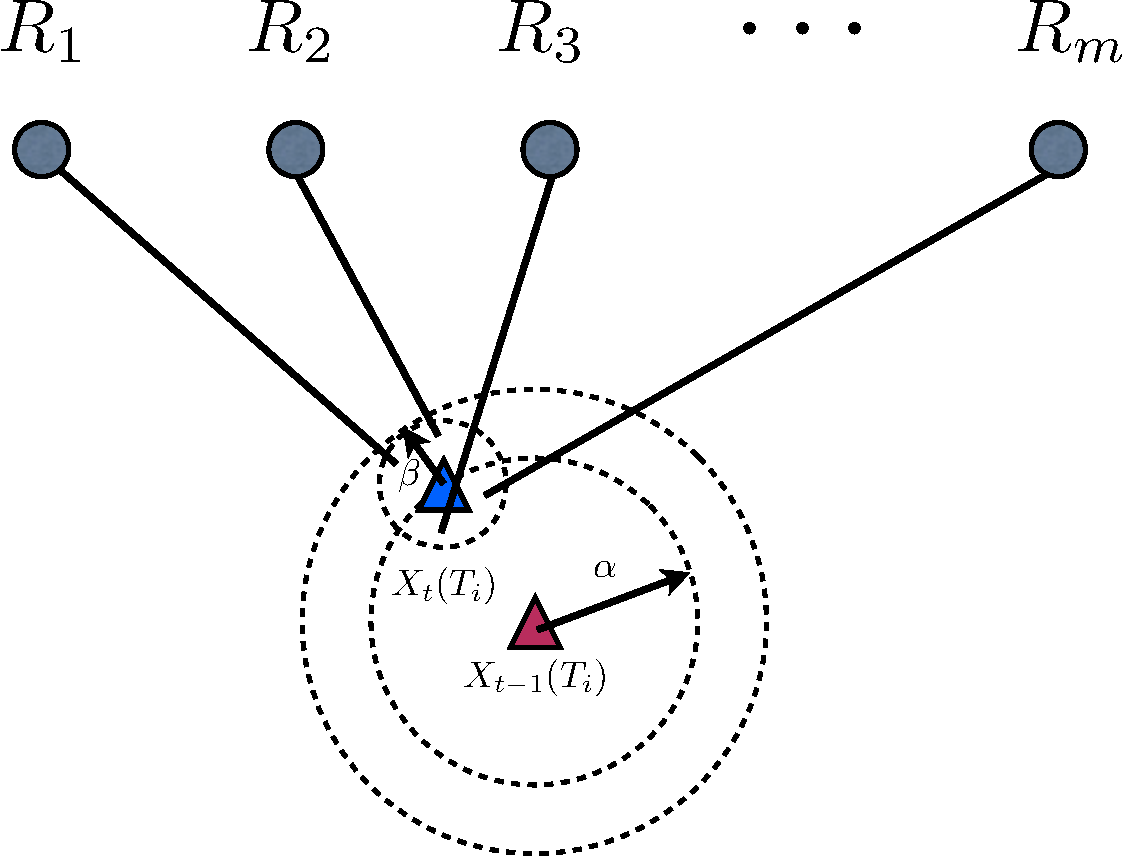
\includegraphics[width=.25\textwidth]{LimitToArrange}
    \end{center}
    \caption{The feasible arrangement can be inferred from last location and ranging
    error }
    \label{fig:LimitToArrange}
\end{figure} 

Theorem \ref{Thm:limit} shows that given $X_{t-1}(T_i)$, all distance with $T_i$ as
origin at time $t$ should be able to touch the disk $(X_{t-1}(T_i),\alpha+\beta)$. This
result can be used to reduce the feasible sub-group.  For each disk
$(X_{t-1}(T_i),\alpha+\beta)$, the distance which can touch  this disk is denoted by
$\tilde{D}_{t}^i$. Obviously $\tilde{D}_{t}^i\subset\tilde{D}_t$. Suppose in
$\tilde{D}_{t}^i$, there are $m^j,j\in[1,n]$ distances which are obtained by receiver
$R_j$. Then the number of assignment containing in $\tilde{D}_{t}^i$ is $N_a^i$, which equals
to: 
 \begin{equation}
     \tilde{N}_a^i=\prod_{j=1}^n m_j 
     \label{equ:nap}
 \end{equation}
Therefore $\tilde{D}_{t}^i$ can contribute $\tilde{N}_a^i$ candidate for $X_{t}(T_i)$.
Because $m_j$ is the number of distance obtained by receiver $j$ whose length is
constrained in small interval, $m_j<m$ with high probability.  We can set
$\hat{X}_{t}(T_i)$ to be the one with maximum likelihood out of $\tilde{N}_a^i$
candidates. Here the likelihood is considered evaluated by taking the validate of
trajectory. We give trajectory with more stable velocity more likelihood, which is
consist with how target move in practice. Technically, this consideration is achieved by
involving particle filter. A Particle $\mathcal{P}_t^k(T_i)$ is a sequence of emitter
$T_i$'s position candidate. For each $T_i$, there are $L$ particle is reserved. Once 
$\tilde{N}_a^i$ position candidate is obtained at $t$, each of $L$ particles is
concatenated with a new position candidate. Totally, $\tilde{N}_a^i\cdot L$ particles
are obtained. These particle are sorted in ascending order of cost function, and only
first $L$ is reserved. Suppose the location reserved in particle $k$ for target $i$ is
denoted by $X'^k_t(T_i)$,The cost function is as follows:
\begin{equation}
    C(\mathcal{P}_t^k(T_i))= ||(X'^k_{t}(T_i)-X'^k_{t-1}(T_i))-(X'^k_{t-1}(T_i)-X'^k_{t-2}(T_i))||
    \label{equ:cost1}
\end{equation}

In this estimation process, $X_{t-1}(T_i)$, the latest historical position of $T_i$,
plays an important role. But $X_{t_1}(T_i)$ is affected by cumulated error.  To
guarantee the accuracy of $X_{t-1}(t_i)$, a accuracy evaluation and reset method is
plugged into the location process. As denoted in figure \ref{fig:DataFlow}, when we got
$X_t(T_i)$, the validation of $X_t(T_i)$ is judged. If the judging result is \emph{Yes},
$X_{t-1}(T_i)$ is updated by $X_t(T_i)$. Otherwise, we think $X_t(T_i)$ is not correct
estimation. A \emph{reset} process is started. In reset process, each emitter is given a
individual timeslot to guarantee the correctness of $X_{t-1}(T_i)$.
\begin{figure}[htpb]
    \begin{center}
	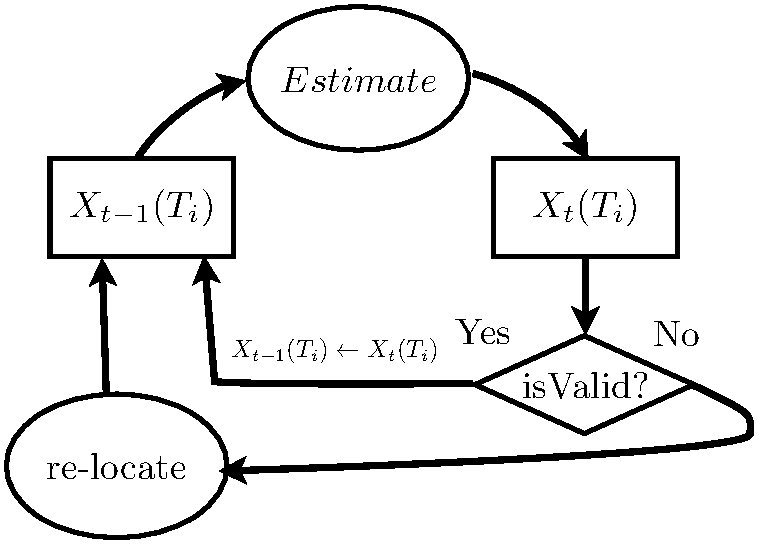
\includegraphics[width=.25\textwidth]{DataFlow}
    \end{center}
    \caption{Plug validation module into locating process}
    \label{fig:DataFlow}
\end{figure}

As a synthesis, the full algorithm for solving equation \ref{equ:ML} is presented. As
this algorithm could support multiple emitter sending their NUP simultaneously, it is
called \emph{UltraChorus}  
\begin{algorithm}[h]
    \caption{UltraChorus}
    \begin{algorithmic}[1]
	\REQUIRE $\tilde{D}_t$ is the set of distance measurement obtained at $t$.
	$X(R_i),i\in[1,n]$ is the location of $n$ receivers. 
	\ENSURE $\{\hat{X}_t(R_i)\},i\in[1,m]$ as the MLE to the location of $R_i,
	i\in[1,m]$.
	\IF {isFirstRound}
	\STATE Reset();
	\STATE isFirstRound $\leftarrow$ FALSE;
	\STATE $\mathcal{P}^k(T_i)\leftarrow\emptyset,\forall i=[1,m],k=[1,L]$ 
	\ENDIF
	\FOR {$i=1,i\le m;i++$} 
	\STATE $\tilde{D}'_t(T_i)=\leftarrow \{d|d\in\tilde{D}_t,||d-|| \}$
	\ENDFOR
    \end{algorithmic}
    \label{algo:LB}
\end{algorithm}
\section{Evaluation}
\section{Conclusion}
%\bibliographystyle{acm}
\bibliographystyle{unsrt}
\bibliography{IPIN}

\end{document}
